\documentclass[margin,line]{res}
\usepackage{hyperref}
\usepackage{url}
\oddsidemargin -.5in
\evensidemargin -.5in
\textwidth=6.0in
\itemsep=0in
\parsep=0in
\topmargin=0in
\topskip=0in
\usepackage{graphicx}
\newenvironment{list1}{
  \begin{list}{\ding{113}}{%
      \setlength{\itemsep}{0in}
      \setlength{\parsep}{0in} \setlength{\parskip}{0in}
      \setlength{\topsep}{0in} \setlength{\partopsep}{0in}
      \setlength{\leftmargin}{0.17in}}}{\end{list}}
\newenvironment{list2}{
  \begin{list}{$\bullet$}{%
      \setlength{\itemsep}{0in}
      \setlength{\parsep}{0in} \setlength{\parskip}{0in}
      \setlength{\topsep}{0in} \setlength{\partopsep}{0in}
      \setlength{\leftmargin}{0.2in}}}{\end{list}}


    
\begin{document}

\name{\LARGE Bharath.T.U} \hfill {\em \today}

\begin{resume}
\section{\sc Contact Information}

\vspace{.05in}
\begin{tabular}{@{}p{3.5in}p{3in}}
2nd  Year B.Tech Student                                                                     & {Phone:}  9497531920 \\
Mar Baselios College Of Engineering
and Technology 
 & {E-mail:}  bharath218usba@gmail.com\\
Mar Ivanios College Rd, Nalanchira.\\
Thattinakam, Thiruvananthapuram, Kerala 695015.\\ 
&
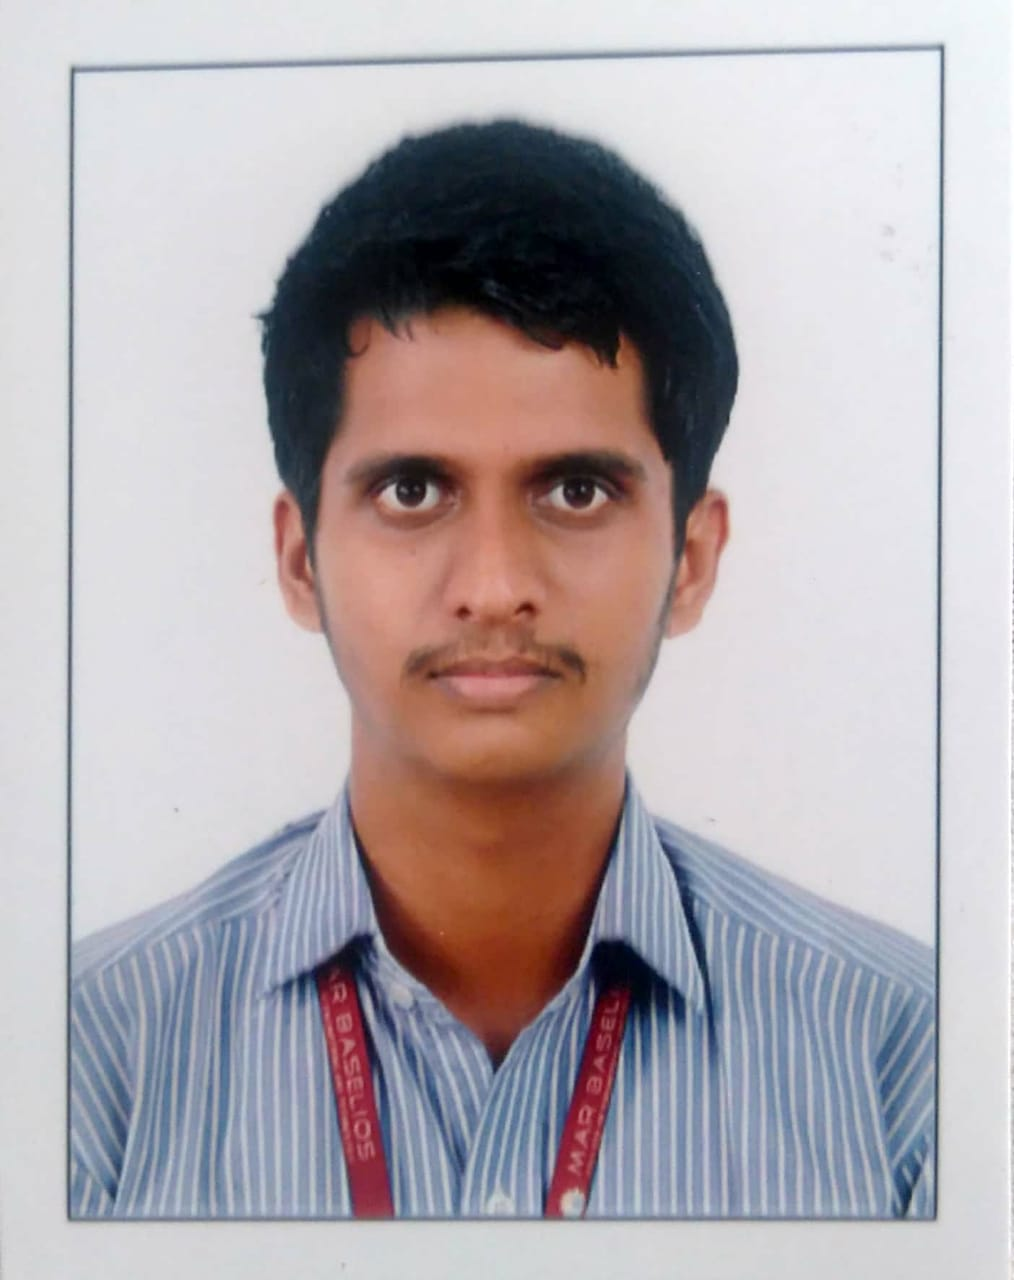
\includegraphics[width=0.1\textheight]{bh}

\end{tabular}

\vspace{.1in}
\section{\sc OBJECTIVE}

To be relevant on the new technologies and have a research or Innovation based career in the field of machine learning , robotics , Iot and networking
\vspace{.1in}
\section{\sc Education}
\begin{tabular}{|l|c|l|c|l|c|}\hline
	\bf Degree&\bf College/School&\bf University&\bf Passing Year&\bf Pass Percentage \\ \hline
	BTech in CSE
	&MBCET & KTU & 2017-Present&1st 2 sem CGPA = 7.68/10 \\ \hline
	Class XII
	&KV-PANGODE & CBSE-AISSCE  & 2017& Overall = 84 Percentage \\&&&&99 Percentage in CS 
	
	\\ \hline
	Class X
	&KV-PANGODE & CBSE-AISSCE  & 2017& Overall = 81.7 Percentage 
	
	\\ \hline
\end{tabular}
\section{\sc PROJECTS}

\begin{enumerate} %Job Description%
	\item omni-directional wheel design \\
	\item Basic implementation of home automation\\
	\item Wireless basket ball count down timer display\\
\end{enumerate}

\section{\sc Training and Internship}
Trained in arduino \\

\end{resume}
\end{document}


